\section{OPQ Mauka}
\label{sec:opq-mauka}

The previous sections discussed the design of OPQ Box, a custom hardware device for collecting four important measures of power quality, and OPQ Makai, a novel, hybrid centralized/decentralized data acquisition scheme which involves two-way communication between the OPQ Boxes.  As a result of these two systems, the OPQ sensor network services will have the ability to collect and analyze high fidelity data about power quality anomalies in a cost-effective, scalable fashion.

There are remaining challenges to creating a useful power quality sensor network. First, the data provided by OPQ Boxes is low-level, "primitive" data consisting of either features (i.e. frequency, voltage, THD, and transients) or waveform data. But what we actually want is actionable insights into grid stability. For example, we might want to know if a given anomalous data value is actually detrimental, or we might wnat to be able to predict when a power quality event might occur in the future based upon the recognition of cyclical events in the historical data.

A second challenge is data volume. Although OPQ Box and OPQ Makai provide a scalable mechanism for communicating power quality data to the cloud services, it is still the case that, over time, a substantial amount of data will accumulate. One strategy is to simply store all of the data sent to the cloud forever. This means that data storage requirements will increase monotonically over time, making the sensor network more costly to maintain the longer it is in place. An alternative strategy is to implement an algorithm to identify uninteresting (or no longer interesting) data and discard it.  Ideally, such an algorithm would enable OPQ sensor network designers to calculate an upper bound on the total amount of cloud storage required as a function of the number of nodes (OPQ Boxes) in the network.

OPQ Mauka addresses both of these issues. First, OPQ Mauka provides a multi-leveled representation for structuring and processing DSN data. The structure and processing at each level is designed with the explicit goal of turning low-level data into actionable insights. Second, each level in the framework implements a "time-to-live" (TTL) strategy for data within the level. This strategy states that data must either progress upwards through the levels towards more abstract, useful representations within a fixed time window, or be discarded and lost forever. The TTL strategy is useful because when implemented, it allows DSN designers to calculate upper bounds on data storage at each level of the framework and supports graceful degradation of DSN performance.

Figure \ref{fig:mauka-data-model} illustrates the hierarchical data model for OPQ Mauka. This data model can be conceptualized as a multi-level hierarchy that adaptively optimizes data storage using a tiered TTL approach and provides a mechanism in which typed aggregated data is continually refined to the point of being of becoming actionable. The data model also includes software components called "actors" that both move data upward through the levels and apply optimizations downward through the levels. Actors are implemented through a plugin architecture, making it easy to experiment with the data model and improve it over time.

\begin{figure}
\center 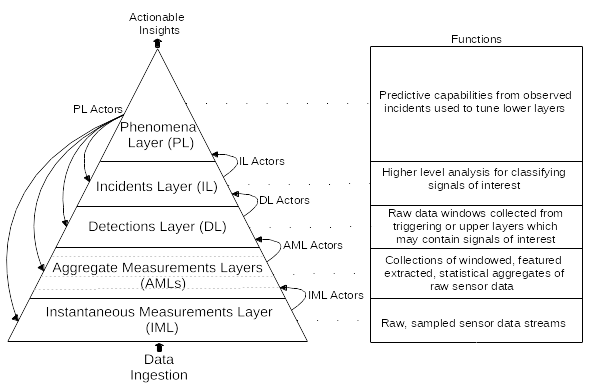
\includegraphics[width=4in]{images/mauka/mauka-data-model.png}
\caption{Mauka data model hierarchy}
\label{fig:mauka-data-model}
\end{figure}

OPQ Mauka sits between OPQ Makai and OPQ’s database. It receives messages from OPQ Makai when it has triggered OPQ Boxes due to something interesting in the low-fidelity data stream. OPQ Mauka then retrieves the raw waveforms stored in the database by OPQ Makai, performs feature extraction, and then forwards the features and/or raw waveform to OPQ Mauka Actors to perform classification and other high level analytics. These results are then stored in the database. Finally, TTL Actors run at predetermined intervals to remove data whose time-to-live has expired.

\subsection{OPQ Mauka Actors}

The current capabilities of OPQ Mauka can be summarized in terms of its Actors, which are implemented as plugins.

{\em BasePlugin.} All Actor plugins derive from the BasePlugin, which provides primitives for running plugins as separate processes, serialization and deserialization of type safe messages, communication over ZeroMQ, metrics collection, MongoDB communication, debugging, and plugin health.

{\em MakaiEventPlugin.} The MakaiEventPlugin Actor is responsible for reading Events newly created by OPQ Makai into OPQ Mauka. It performs feature extraction on the raw Event data streams and forwards those features (or the raw data) to subscribing plugins. This allows OPQ Mauka to perform feature extraction once, and reuse those features in multiple plugins.

{\em FrequencyVariationPlugin.} The FrequencyVariationPlugin is used to classify generic fre- quency sags, swells, and interruptions as defined by the IEEE1159 standard[29]. Both duration and deviation from nominal are used to perform these classifications. Duration classifications in- clude frequency deviations that last for less than 50 ns, between 50 ns to 1 ms, and 1 ms to 50 ms. Classifications for deviations from nominal are performed for values that are up to 40% deviation
     49

     nominal. The plugin subscribes to messages from the “WindowedFrequency” topic which includes a payload of frequency features over one electrical cycle.
     When a message is received, the plugin uses configurable thresholds to find frequency fluctu- ations within the windowed frequency streams. The plugin is able to classify frequency swells, frequency interruptions, and frequency sags. When a new frequency variation is detected, a fre- quency Incident is created



